\documentclass[12pt, a5paper]{jarticle}
\usepackage[utf8]{inputenc}
\usepackage{amsmath}
\usepackage{amsfonts}
\usepackage{amssymb}
\usepackage{graphicx}
%\usepackage[dvipdfmx]{graphicx} % グラフィクスを使うためのパッケージ
\usepackage[dvipdfmx]{color}
\usepackage[left=2.00cm,right=2.00cm,top=2.5cm]{geometry}
\usepackage{array}
\usepackage{caption}
\usepackage{colortbl,array,xcolor}
\usepackage{here}
\usepackage{multicol}
\usepackage{multirow}
\usepackage{okumacro}
\usepackage{pxrubrica} 				%ルビを振る為
\usepackage{setspace}
\usepackage{ascmac}
\usepackage{fancybox}
\usepackage{longtable}
\usepackage{booktabs}
\usepackage{colortbl,array,xcolor}
\usepackage{wrapfig}	%
\usepackage{paralist}	%
\captionsetup[figure]{font=scriptsize,labelfont=scriptsize}

\title{旅行のしおり}
\author{}
\date{\empty}

\begin{document}
	%目次の出力
	\renewcommand{\thepage}{\roman{page}}
	\setcounter{page}{1}
	
	\tableofcontents
	\clearpage
	
	\renewcommand{\thepage}{\arabic{page}}
	\setcounter{page}{1}
	\begin{center}
	\section*{\underline{\fontsize{45pt}{20pt}\selectfont 本旅行の目的}}
\end{center}
\vspace{1.5cm}

\begin{itemize}
	\item[〇]お泊まりということで非日常的な体験を通じて親睦をより深いものとする.\\\\
	\item[〇]sample text\\\\
	\item[〇]sample text\\\\
	\item[◎]悔いの残らないよう全力で楽しみ素晴らしい思い出の1ページとして記憶に綴る.\\\\
\end{itemize}




	\addcontentsline{toc}{section}{本旅行の目的}
	\newpage
	%\section{持ち物チェック}
\vspace{1em}
\subsection*{スーツケース}
\addcontentsline{toc}{subsection}{カバン(大)}
\begin{table}[htb]
	\centering
	\begin{tabular}{|Wl{5cm}|Wc{1cm}|Wc{1.5cm}|Wc{1.5cm}|} \hline
		\rowcolor[rgb]{0.7,0.9,1.0}
		\multicolumn{1}{|c|}{入れる物} & 数 & \multicolumn{2}{c|}{チェック欄}\\ \hline
		着替え & 2 & □ & □ \\ \hline
		靴下 & 2 & □ & □ \\ \hline
		下着 & 3 & □ & □ \\ \hline
		コンタクトケース,洗浄液 & 1 & □ & □ \\ \hline
		カラコン & 2 & □ & □ \\ \hline
		スキンケアセット & 1 & □ & □ \\ \hline
		薬 & 2 & □ & □ \\ \hline
		袋 & 2 & □ & □ \\ \hline
		ヘアアイロン & 1 & □ & □ \\ \hline
		ヘアトリートメント& 1 & □ & □ \\ \hline
		メガネ & 1 & □ & □ \\ \hline
		メイク道具一式 & 1 & □ & □ \\ \hline
		筆記用具(ペン・消しゴム) & 1 & □ & □ \\ \hline
		アクセサリー類 &  & □ & □ \\ \hline
		エコバッグ & 1 & □ & □ \\ \hline
		折りたたみ傘 & 1 & □ & □ \\ \hline
		iPad mini & 1 & □ & □ \\ \hline
		充電器 & 1 & □ & □ \\ \hline
		延長コード & 1 & □ & □ \\ \hline
	\end{tabular}
	
\end{table}
\newpage
\vspace{1em}
\subsection*{手荷物}
\addcontentsline{toc}{subsection}{カバン(小)}
\begin{table}[htb]
	\centering
	\begin{tabular}{|Wl{5cm}|Wc{1cm}|Wc{1.5cm}|Wc{1.5cm}|} \hline
		\rowcolor[rgb]{0.7,0.9,1.0}
		\multicolumn{1}{|c|}{入れる物} & 数 & \multicolumn{2}{c|}{チェック欄}\\ \hline
		財布 & 1 & □ & □ \\ \hline
		携帯電話 & 1 & □ & □ \\ \hline
		ハンカチ・ティッシュ & 1 & □ & □ \\ \hline
		自撮り棒 & 1 & □ & □ \\ \hline
		これ & 1 & □ & □ \\ \hline
		マスク & 3 & □ & □ \\ \hline
		ヘアアクセサリー & 1 & □ & □ \\ \hline
		メイク道具(携帯用) & 1 & □ & □ \\ \hline
		モバイルバッテリー & 1 & □ & □ \\ \hline
		鎮痛剤 & 4 & □ & □ \\ \hline
		リップクリーム & 1 & □ & □ \\ \hline
		ブラシ & 1 & □ & □ \\ \hline
		&  & □ & □ \\ \hline
		&  & □ & □ \\ \hline
		&  & □ & □ \\ \hline
		&  & □ & □ \\ \hline
		&  & □ & □ \\ \hline
		&  & □ & □ \\ \hline
	\end{tabular}
	
\end{table}
\vspace{2em}
\begin{center}
	\underline{\Huge 忘れ物に気を付けましょう}
\end{center}

	%\section{持ち物チェック}
\vspace{1em}
\subsection*{カバン(大)}
\addcontentsline{toc}{subsection}{カバン(大)}
\begin{table}[htb]
	\centering
	\begin{tabular}{|Wl{5cm}|Wc{1cm}|Wc{1.5cm}|Wc{1.5cm}|} \hline
		\rowcolor[rgb]{0.7,0.9,1.0}
		\multicolumn{1}{|c|}{入れる物} & 数 & \multicolumn{2}{c|}{チェック欄}\\ \hline
		着替え              & 2 & □ & □ \\ \hline
		靴下               & 3 & □ & □ \\ \hline
		下着                & 3 & □ & □ \\ \hline
		薬                  & 4 & □ & □ \\ \hline
		袋                  & 2 & □ & □ \\ \hline
		専用プロテクター    & 1 & □ & □ \\ \hline
		充電器              & 2 & □ & □ \\ \hline
		&  & □ & □ \\ \hline
		&  & □ & □ \\ \hline
		&  & □ & □ \\ \hline
		&  & □ & □ \\ \hline
		&  & □ & □ \\ \hline
		&  & □ & □ \\ \hline
		&  & □ & □ \\ \hline
		&  & □ & □ \\ \hline
		&  & □ & □ \\ \hline
		&  & □ & □ \\ \hline
		&  & □ & □ \\ \hline
		&  & □ & □ \\ \hline
	\end{tabular}
	
\end{table}
\newpage
\vspace{1em}
\subsection*{カバン(小)}
\addcontentsline{toc}{subsection}{カバン(小)}
\begin{table}[htb]
	\centering
	\begin{tabular}{|Wl{5cm}|Wc{1cm}|Wc{1.5cm}|Wc{1.5cm}|} \hline
		\rowcolor[rgb]{0.7,0.9,1.0}
		\multicolumn{1}{|c|}{入れる物} & 数 & \multicolumn{2}{c|}{チェック欄}\\ \hline
		財布                & 1 & □ & □ \\ \hline
		携帯電話            & 1 & □ & □ \\ \hline
		iPadAir             & 1 & □ & □ \\ \hline
		ハンカチ            & 1 & □ & □ \\ \hline
		ティッシュ          & 1 & □ & □ \\ \hline
		これ                & 1 & □ & □ \\ \hline
		マスク              & 3 & □ & □ \\ \hline
		除菌シート          & 1 & □ & □ \\ \hline
		例のやつ            & 1 & □ & □ \\ \hline
		モバイルバッテリー  & 1 & □ & □ \\ \hline
		筆記用具            & 1 & □ & □ \\ \hline
		ICカード            & 1 & □ & □ \\ \hline
		ミニバッグ          & 1 & □ & □ \\ \hline
		折り畳み傘          & 1 & □ & □ \\ \hline
		&  & □ & □ \\ \hline
		&  & □ & □ \\ \hline
		&  & □ & □ \\ \hline
		&  & □ & □ \\ \hline
	\end{tabular}
	
\end{table}
\vspace{2em}
\begin{center}
	\underline{\Huge 忘れ物に気を付けましょう}
\end{center}

	\newpage
	\begin{center}
	\section*{\underline{\fontsize{45pt}{20pt}\selectfont 旅行の心得}}
\end{center}
\vspace{1.5cm}
\begin{description}
	\item[\huge 『ゆったりと』]\mbox{}\\
	普段から旅の移動効率化などを図っているが,忙しさは時として旅の安寧を損ねる.
	ゆとりを持ったスケジュールの上で行動することで,思わぬ事象と巡り合うこともまた旅の一興である.\\\\
	\item[\huge 『社会人としての振舞い』]\mbox{}\\
	我々は新卒ではあるものの社会人1年目であり,学生ではない.
	経済的にも精神的にも自立し始めているが,それに驕らず旅先では節度ある行動をすべきである.\\\\
	\item[\huge 『食道楽』]\mbox{}\\
	\ruby{食道楽}{くいどうらく}とは,美味しいものを食べたり料理を作ったりすることに熱中し,それを生き甲斐にすることである.
	旅行ではその地域ならではの食材や料理を目にすることがある.
	非日常を経験する要素に,その旅先固有の食事を楽しむことも含まれるだろう.
\end{description}
	\addcontentsline{toc}{section}{旅行の心得}
	\newpage
	%\section{旅行日程}
\subsection*{2月9日(日) 第1日目}
\addcontentsline{toc}{subsection}{2月10日(金) 第0日目}
\begin{longtable}{|Wc{1cm}|Wl{3.5cm}|Wl{5.5cm}|} \hline
	\rowcolor[rgb]{1.0,1.0,0.7}
	\textbf{時刻} & \multicolumn{1}{c|}{\textbf{行程}} & \multicolumn{1}{c|}{\textbf{内容}}\\ \hline
	:   & \footnotesize{起床} & \scriptsize{おはよう} \\ \hline
	:   & \footnotesize{支度} & \scriptsize{持ち物最終チェック(司温は修論発表会を聞く前)}\\ \hline
	14:35 & \footnotesize{出発} & \scriptsize{遅延情報を確認しながら行動}\\ \hline
	14:51 & \footnotesize{北岡崎駅 発} & \scriptsize{愛知環状鉄道 岡崎行・1番線} \\ 
	14:59 & \footnotesize{愛環岡崎駅 着} & \scriptsize{愛知環状鉄道・0番線(230円)} \\ \hline
	15:12 & \footnotesize{JR岡崎駅 発} & \scriptsize{JR東海道本線新快速 大垣行・3番線} \\ 
	15:38 & \footnotesize{JR金山駅 着} & \scriptsize{JR東海道本線・6番線(620円)} \\ \hline
	15:49 & \footnotesize{名鉄金山駅 発} & \scriptsize{名鉄名古屋本線準急 中部国際空港行・3.4番線} \\ 
	16:33 & \footnotesize{中部国際空港駅 着} & \scriptsize{名鉄名古屋本線準急 中部国際空港行 (830円)} \\ \hline
	16:40 & \footnotesize{中部国際空港 着} & \scriptsize{徒歩} \\ \hline
	17:45 & \footnotesize{中部国際空港 発} & \scriptsize{搭乗手順 p.10 参照} \\ 
	19:20 & \footnotesize{長崎空港 着} & \scriptsize{} \\ \hline
	19:40 & \footnotesize{長崎空港駅 発} & \scriptsize{長崎県営バス 諫早駅前行} \\
	19:49 & \footnotesize{古町駅 着} & \scriptsize{(210円)} \\ \hline
	20:00 & \footnotesize{君の家食堂} & \scriptsize{皿うどん} \\ \hline
	21:00 & \scriptsize{チサンイン大村長崎空港 着} & \scriptsize{チェックイン} \\
	21:30 & \footnotesize{入浴} & \scriptsize{} \\
	23:00 & \footnotesize{就寝} & \scriptsize{おやすみ} \\
	\hline
\end{longtable}
\newpage

\subsection*{2月10日(月) 第2日目}
\addcontentsline{toc}{subsection}{2月11日(土) 第1日目}
\begin{longtable}{|Wc{1cm}|Wl{3.5cm}|Wl{5.5cm}|} \hline
	\rowcolor[rgb]{1.0,1.0,0.7}
	\textbf{時刻} & \multicolumn{1}{c|}{\textbf{行程}} & \multicolumn{1}{c|}{\textbf{内容}}\\ \hline
	07:00 & \footnotesize{起床} & \scriptsize{おはよう} \\
	08:00 & \footnotesize{支度} & \scriptsize{忘れ物確認}\\ \hline
	09:50 & \scriptsize{チサンイン大村長崎空港 発} & \scriptsize{チェックアウト}\\
	10:20 & \footnotesize{大村駅 着} & \scriptsize{徒歩} \\ \hline
	10:27 & \footnotesize{大村駅 発} & \scriptsize{JR区間快速シーサイドライナー 長崎行}\\
	11:08 & \footnotesize{長崎駅 着} & \scriptsize{JR区間快速シーサイドライナー 長崎行(760円)}\\ \hline
	11:20 & \footnotesize{長崎市観光案内所} & \scriptsize{電車1日乗車券を購入(600円)}\\ \hline	
	11:31 & \footnotesize{長崎駅前駅 発} & \scriptsize{\color{blue}{長崎電気軌道 1系統 崇福寺行}}\\
	11:35 & \footnotesize{出島駅 着} & \scriptsize{}\\ \hline
	11:40 & \footnotesize{出島} & \scriptsize{所要時間:30分程度 入場料:520円} \\ \hline
	12:14 & \footnotesize{出島駅 発} & \scriptsize{\color{blue}{長崎電気軌道 1系統 崇福寺行}} \\
	12:17 & \footnotesize{新地中華街駅 着} & \scriptsize{} \\ \hline
	12:20 & \footnotesize{新地中華街} & \scriptsize{食べ歩きで昼食} \\ \hline
	12:58 & \footnotesize{新地中華街駅 発} & \scriptsize{\textcolor{green}{長崎電気軌道 5系統 蛍茶屋行}} \\ 
	13:04 & \footnotesize{めがね橋駅 着} & \scriptsize{} \\ \hline 
	13:07 & \footnotesize{眼鏡橋} & \scriptsize{ハートストーンが有名らしい} \\ \hline
	13:22 & \footnotesize{市役所駅 発} & \scriptsize{\textcolor{red}{長崎電気軌道 3系統 赤迫行}} \\
	13:38 & \footnotesize{原爆資料館駅 着} & \scriptsize{} \\ \hline
	13:45 & \footnotesize{原爆資料館} & \scriptsize{所要時間:1時間程度 入館料:200円} \\ \hline
	14:55 & \footnotesize{原爆資料館駅 発} & \scriptsize{\textcolor{blue}{1系統 崇福寺行} または \textcolor{red}{3系統 蛍茶屋行}} \\
	14:57 & \footnotesize{浦上駅前駅 着} & \scriptsize{} \\ \hline
	15:11 & \footnotesize{浦上駅 発} & \scriptsize{JR区間快速シーサイドライナー 佐世保行} \\
	16:36 & \footnotesize{ハウステンボス駅 着} & \scriptsize{区間快速シーサイドライナー 佐世保行(1500円)} \\ \hline
	17:00 & \footnotesize{ハウステンボス 着} & \scriptsize{アフター5パスポート} \\ \hline
	17:10 & \footnotesize{入国・手荷物預かり所 発} & \scriptsize{専用バス(最悪歩けば良い)} \\ \hline
	17:20 & \footnotesize{ホテルアムステルダム} & \scriptsize{チェックイン} \\ \hline
	18:00 & \footnotesize{夕飯} & \scriptsize{園内で長崎ちゃんぽんを食べたい} \\ \hline
	21:00 & \footnotesize{Bar} & \scriptsize{ホテル内にある} \\
	21:30 & \footnotesize{入浴} & \scriptsize{} \\ 
	22:30 & \footnotesize{日記記入} & \scriptsize{} \\ 
	23:00 & \footnotesize{就寝} & \scriptsize{おやすみ} \\ \hline
\end{longtable}
\newpage

\subsection*{2月11日(火) 第3日目}
\addcontentsline{toc}{subsection}{2月12日(日) 第2日目}
\begin{longtable}{|Wc{1cm}|Wl{3.5cm}|Wl{5.5cm}|} \hline
	\rowcolor[rgb]{1.0,1.0,0.7}
	\textbf{時刻} & \multicolumn{1}{c|}{\textbf{行程}} & \multicolumn{1}{c|}{\textbf{内容}}\\ \hline
	07:30 & \footnotesize{起床} & \scriptsize{おはよう} \\ \hline
	08:00 & \footnotesize{支度} & \scriptsize{}\\ \hline
	09:00 & \footnotesize{ハウステンボス 散策開始} & \scriptsize{} \\ 
	11:00 & \footnotesize{ナインチェカフェ} & \scriptsize{混むのでなるべく早めに} \\
	& \footnotesize{カステラの城} & \scriptsize{カステラ買う} \\
	& \footnotesize{} & \scriptsize{} \\
	& \footnotesize{} & \scriptsize{} \\
	& \footnotesize{} & \scriptsize{} \\
	& \footnotesize{} & \scriptsize{} \\
	17:30 & \footnotesize{\ruby{戎}{えびす}座} & \scriptsize{5周年のお祝い} \\
	& \footnotesize{} & \scriptsize{} \\ \hline
	21:30 & \footnotesize{入浴} & \scriptsize{} \\ 
	22:30 & \footnotesize{日記記入} & \scriptsize{} \\ 
	23:00 & \footnotesize{就寝} & \scriptsize{おやすみ} \\ \hline
\end{longtable}
\vspace{4em}
\begin{center}
	\underline{\LARGE{お家に帰るまでが旅行です。}}
\end{center}

	\newpage
	%\section{行程詳細}
\vspace{1em}
\subsection*{航空券}
\addcontentsline{toc}{subsection}{航空券}
\begin{table}[htb]
	\centering
	%\begin{tabular}{Wc{2cm}Wr{3.5cm}Wr{3.5cm}}
	\begin{tabular}{crr}
		\toprule
		&  \multicolumn{1}{c}{\textbf{行き}} &  \multicolumn{1}{c}{\textbf{帰り}}\\
		\midrule
		\rowcolor{lightgray!20}
		\multicolumn{1}{c|}{\textbf{日時}}     & 2月10日(金) & 2月13日(月)\\ 
		\multicolumn{1}{c|}{\textbf{便名}} & ANA373 & ANA374\\
		\rowcolor{lightgray!20}
		\multicolumn{1}{c|}{\textbf{出発}} & 中部国際 17:45 & 長崎 20:00 \\
		\multicolumn{1}{c|}{\textbf{到着}} & 長崎 19:20 & 中部国際 21:10\\
		\rowcolor{lightgray!20}
		\multicolumn{1}{c|}{\textbf{席1}} & 25B & 28H\\ 
		\multicolumn{1}{c|}{\textbf{席2}} & 25C & 28J\\
		\rowcolor{lightgray!20}
		\multicolumn{1}{c|}{\textbf{確認番号}} & 698029292 & 418051105\\
		\bottomrule
	\end{tabular}
\end{table}
\vspace{2em}

\subsection*{搭乗手順}
\addcontentsline{toc}{subsection}{搭乗手順}
\begin{enumerate}
	\item
	オンラインチェックイン(ANAアプリ,出発の24時間前から)
	\item
	モバイル搭乗券発行(ANAアプリ,出発の20分前までに)
	\item 保安検査場の通過(出発の20分前までに)
	\item 搭乗口の通過(出発の10分前までに)
\end{enumerate}
	\newpage
	%\section{各詳細}
\subsection*{松島}
\addcontentsline{toc}{subsection}{松島}
\footnotesize

\textbf{松島}は,仙台市から車で約30分ほどの距離に位置する美しい観光地で,特にその景観と歴史的な価値で知られている.
松島は日本三景の一つに数えられ,数百の小島が点在する風光明媚な海岸線が特徴である.

\begin{figure}[H]
	\centering
	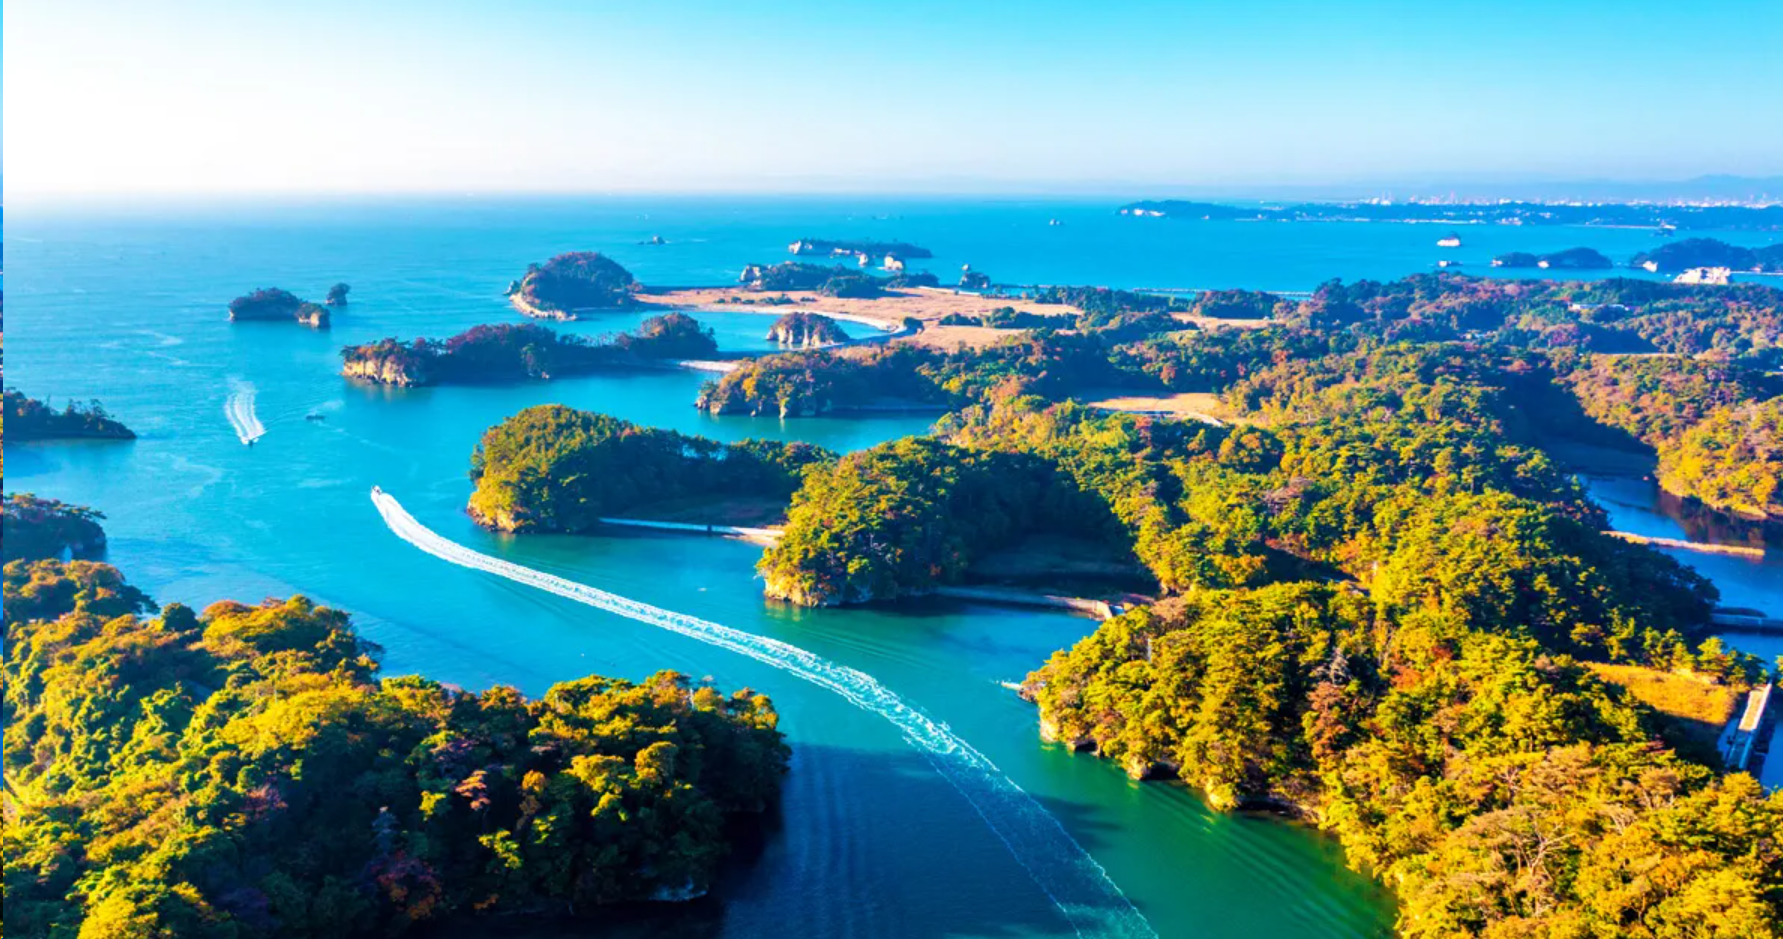
\includegraphics[width=0.7\linewidth]{img/matsushima-islets}
	\label{fig:matsushima-islets}
\end{figure}

松島の最大の魅力は,その景観である.
松島湾には約260の小島があり,四季折々の風景が楽しめる.
特に秋の紅葉や冬の雪景色は別格であり,多くの観光客が訪れる.
松島の景観は,松の木々と海の青さが織りなすコントラストが美しく,訪れる人々を魅了する.

\begin{figure}[H]
	\centering
	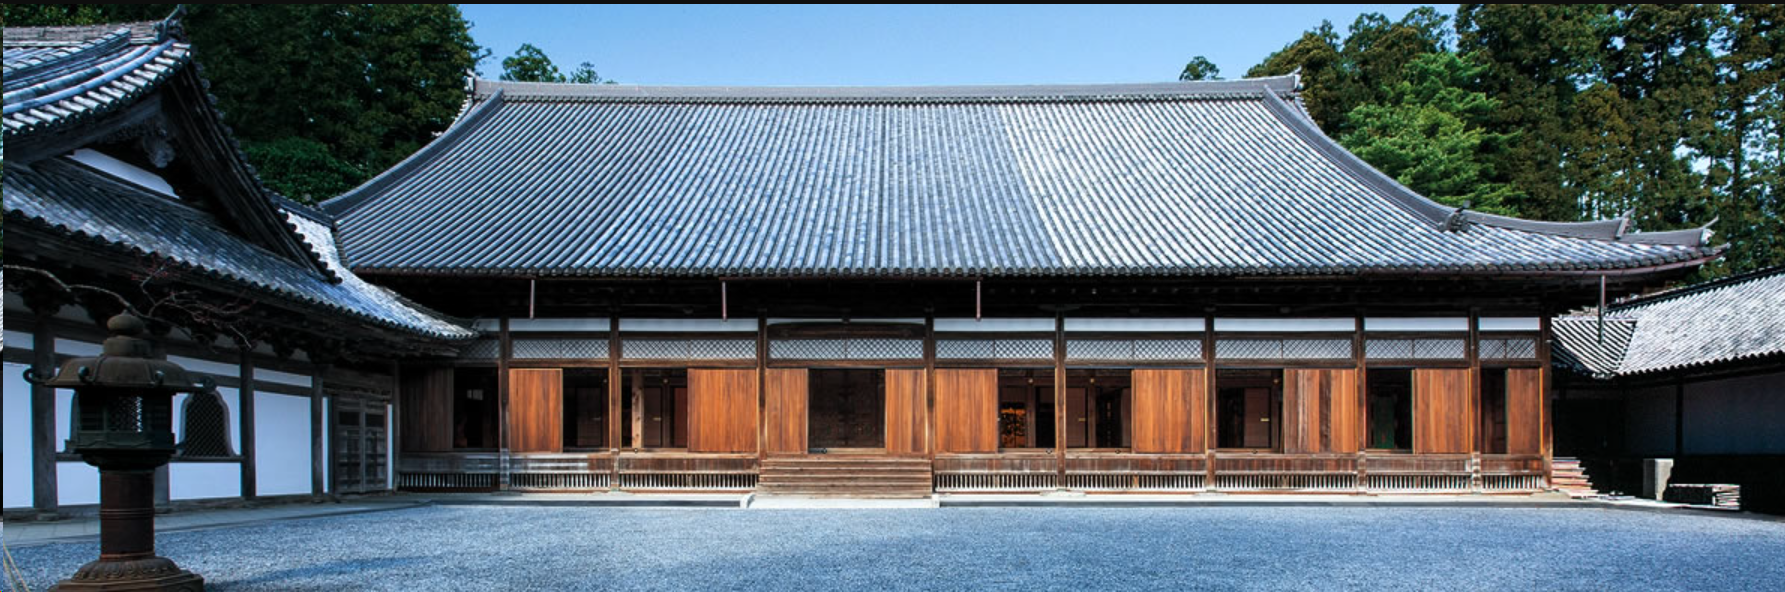
\includegraphics[width=0.8\linewidth]{img/zuiganji}
	\label{fig:zuiganji}
\end{figure}

松島には多くの歴史的名所がある.
とくに有名なものに,松島のシンボルともいえる\textbf{五大堂}がある.
この堂は松島の景観を一望できる場所に位置し,観光客に人気のスポットである.
また,松島には\textbf{\ruby{瑞巌寺}{ずいがんじ}}という重要文化財もあり,歴史的な建物や庭園が見どころだ.
\newpage

\subsection*{大崎八幡宮}
\addcontentsline{toc}{subsection}{大崎八幡宮}

\textbf{大宮八幡宮}は平安時代の初期に創建されたとされ,長い歴史を持つ神社である.
神社の主祭神は\ruby{八幡神}{やはたのかみ}であり,武運や商売繁盛を祈願するために多くの人が訪れる.
また,神社の建物は江戸時代に再建されたもので,豪華な装飾や彫刻が施されている.
特に,重要文化財に指定されている本殿は見事な技術で作られており,訪れる人々を魅了する.

大崎八幡宮では,年間を通じてさまざまな祭りや行事が行なわれる.
とくに有名なのは,毎年行なわれる\textbf{大崎八幡宮例大祭}で,地元の人々や観光客が集まり,\ruby{神輿}{しんよ}\footnote{神社で行なわれるお祭りの際に神霊を載せて担ぐ乗り物.\ruby{御輿}{みこし}とも呼ばれる.} や伝統的な踊りが披露される.
また,初詣や七五三,結婚式など,個人の祈願や祝い事にも利用され,多くの人々に親しまれている.
\begin{figure}[H]
	\centering
	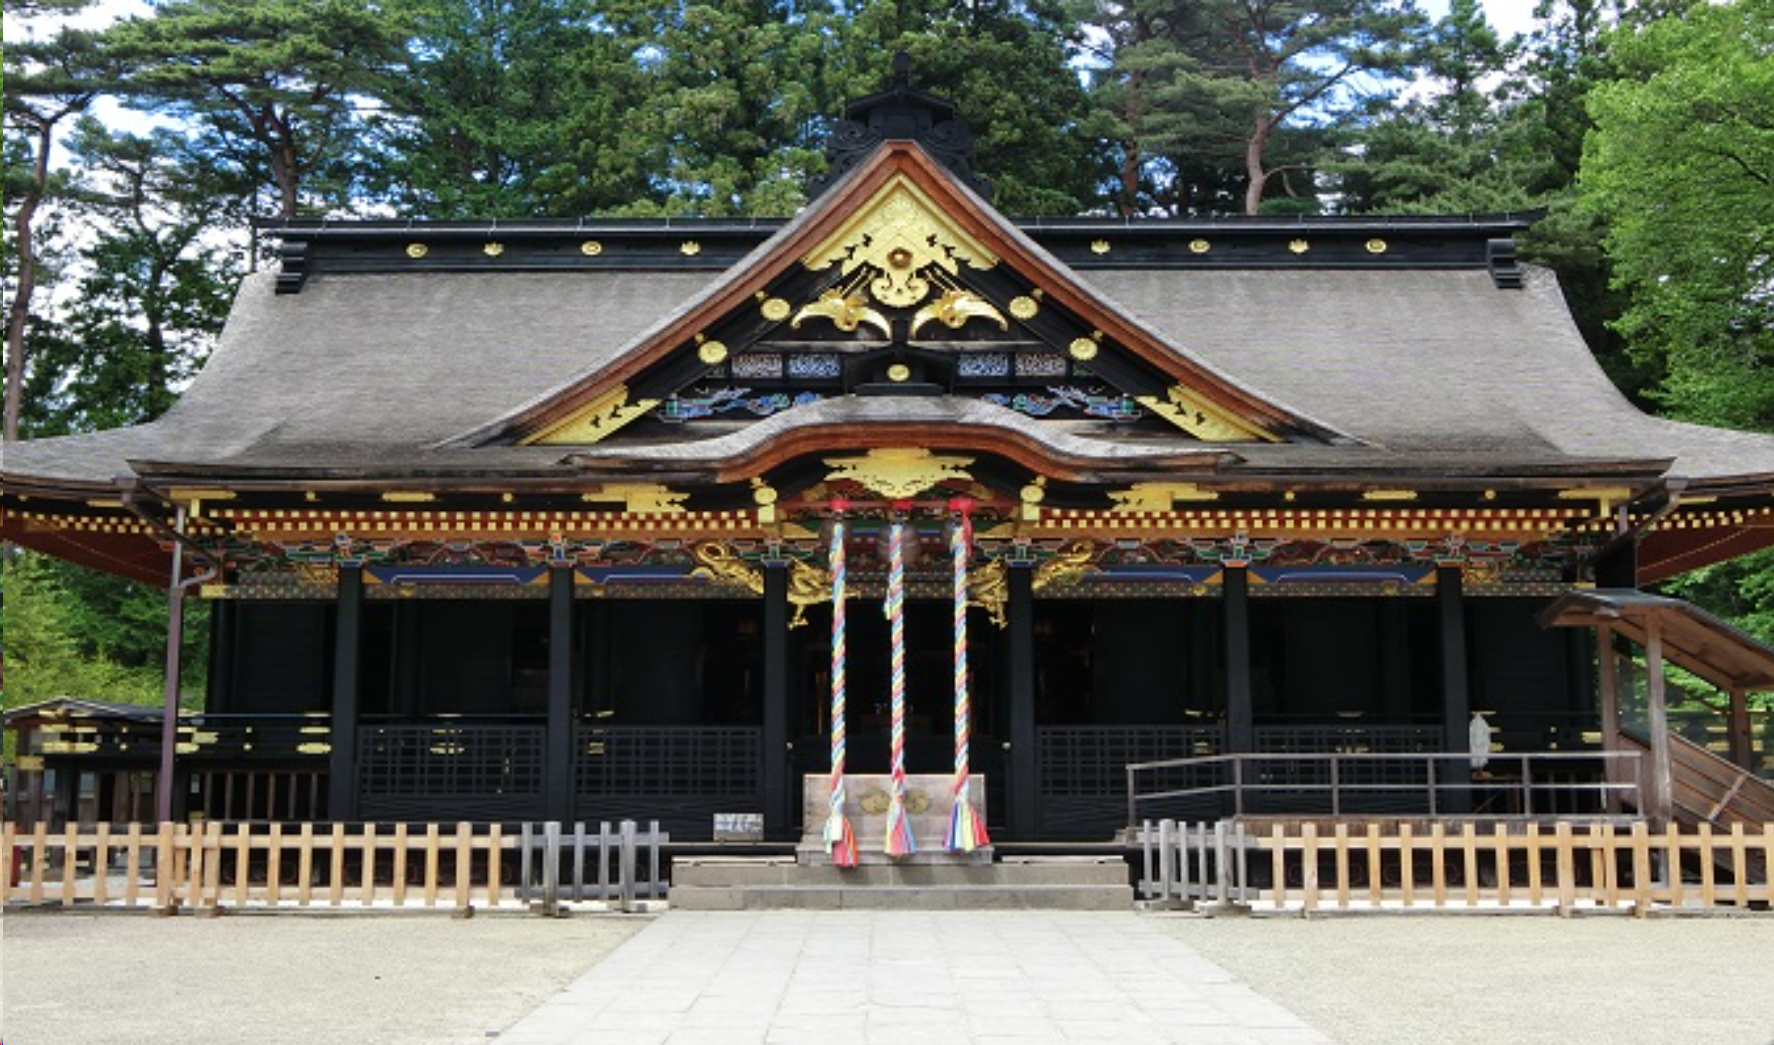
\includegraphics[width=0.8\linewidth]{img/osakimachimangu}
	\label{fig:osakimachimangu}
\end{figure}

大崎八幡宮は,歴史的な価値と自然の美しさを兼ね備えた場所であり,訪れる人々にとって特別な体験を提供している.
神社の静かな雰囲気の中,心を落ち着け,祈りをささげることができる貴重なスポットである.
ぜひ一度訪れて,その魅力を体感してみるとよい.
\newpage

\subsection*{伊達政宗}
\addcontentsline{toc}{subsection}{伊達政宗}

\begin{figure}[H]
	\centering
	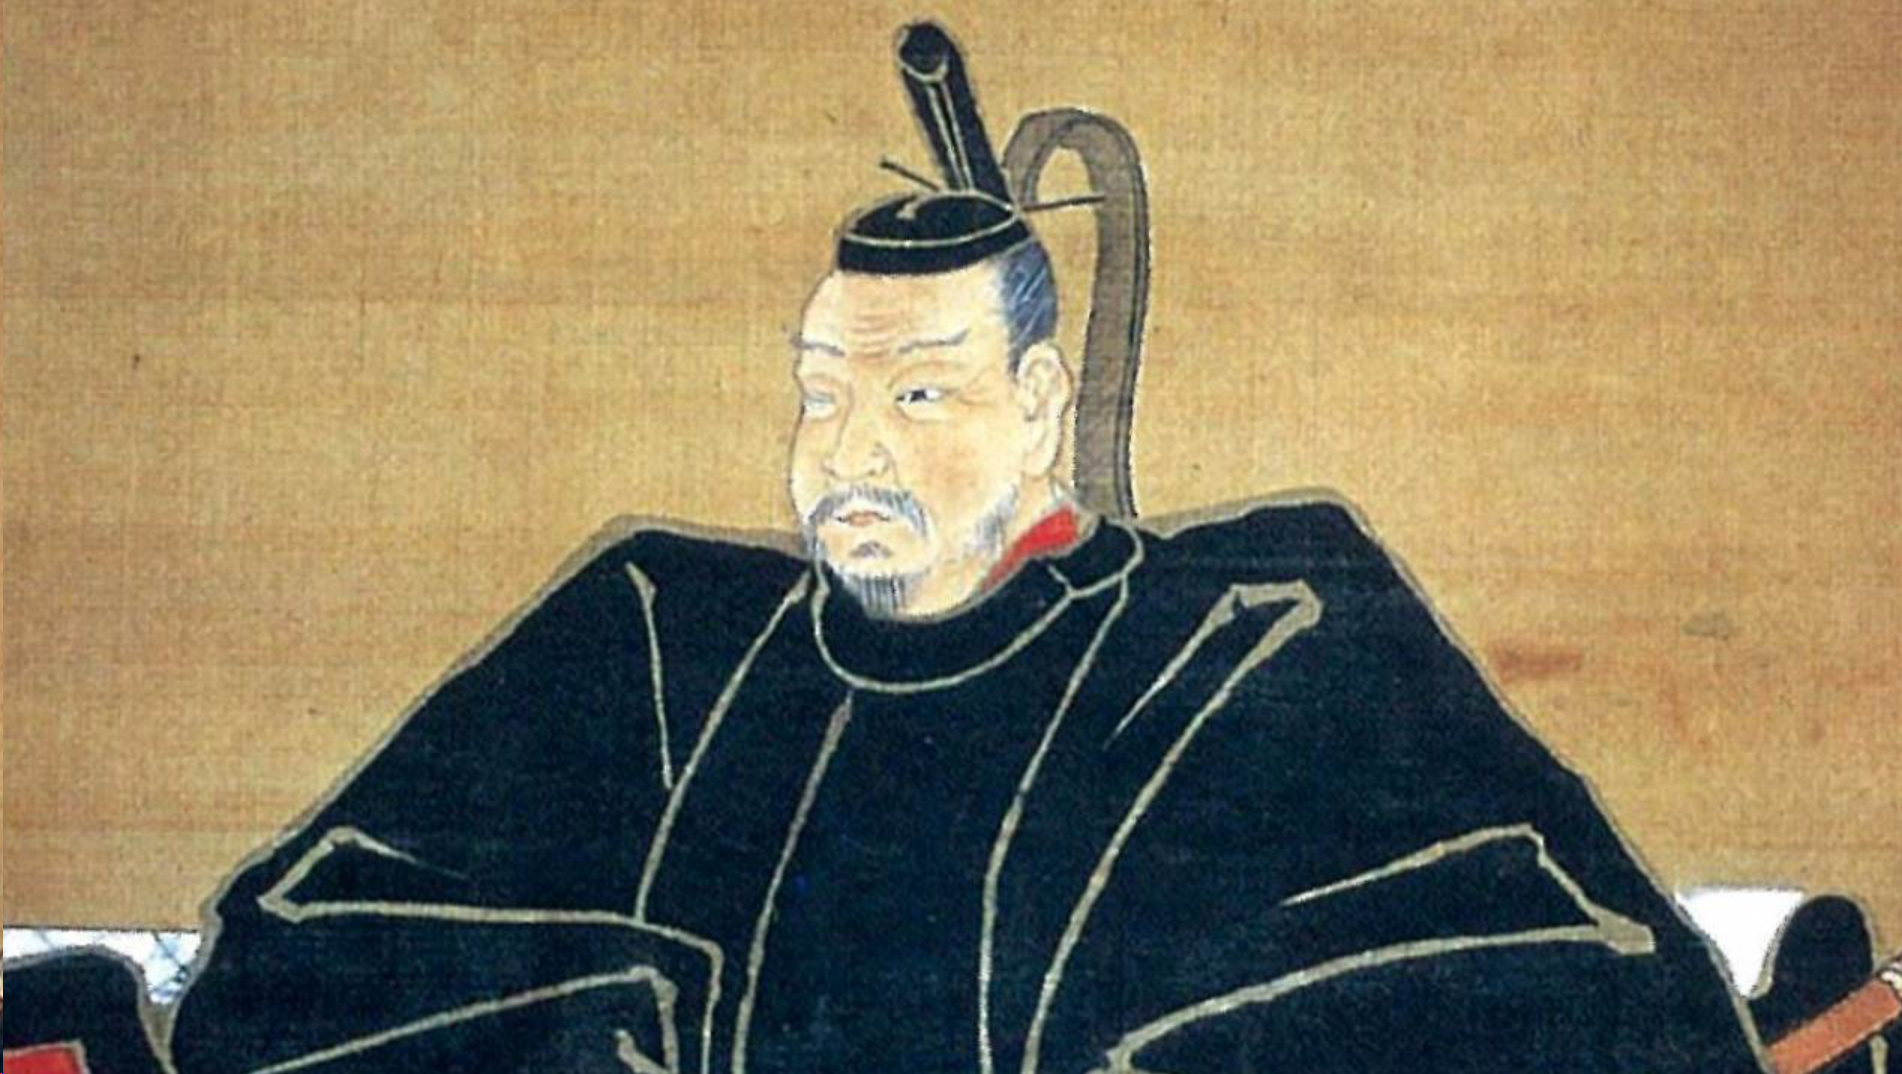
\includegraphics[width=0.7\linewidth]{img/datemasamune}
	\label{fig:datemasamune}
\end{figure}


\textbf{伊達政宗}は戦国時代の日本の著名な武将であり,特に東北地方の支配者として知られる.
1521年に生まれ1590年に亡くなるまでの間に,独自の政治的手腕と軍事的才能を発揮した.
政宗は,特にその戦略的な思考と外交能力で知られ,彼の治世下で仙台藩を築き上げた.

政宗は,幼少期に片目を失ったことから,\textbf{独眼竜}と呼ばれるようになった.
彼は,父である伊達\ruby{輝宗}{てるむね}の後を継ぎ,家族の名声を高めるために多くの戦闘に参加した.
政宗は周囲の大名との同盟を結び,また敵対する勢力に対しても果敢に戦った.
特に,彼は豊臣秀吉の下での戦いに参加し,その後の関ケ原の戦いにも影響を与えた.

\begin{figure}[H]
	\centering
	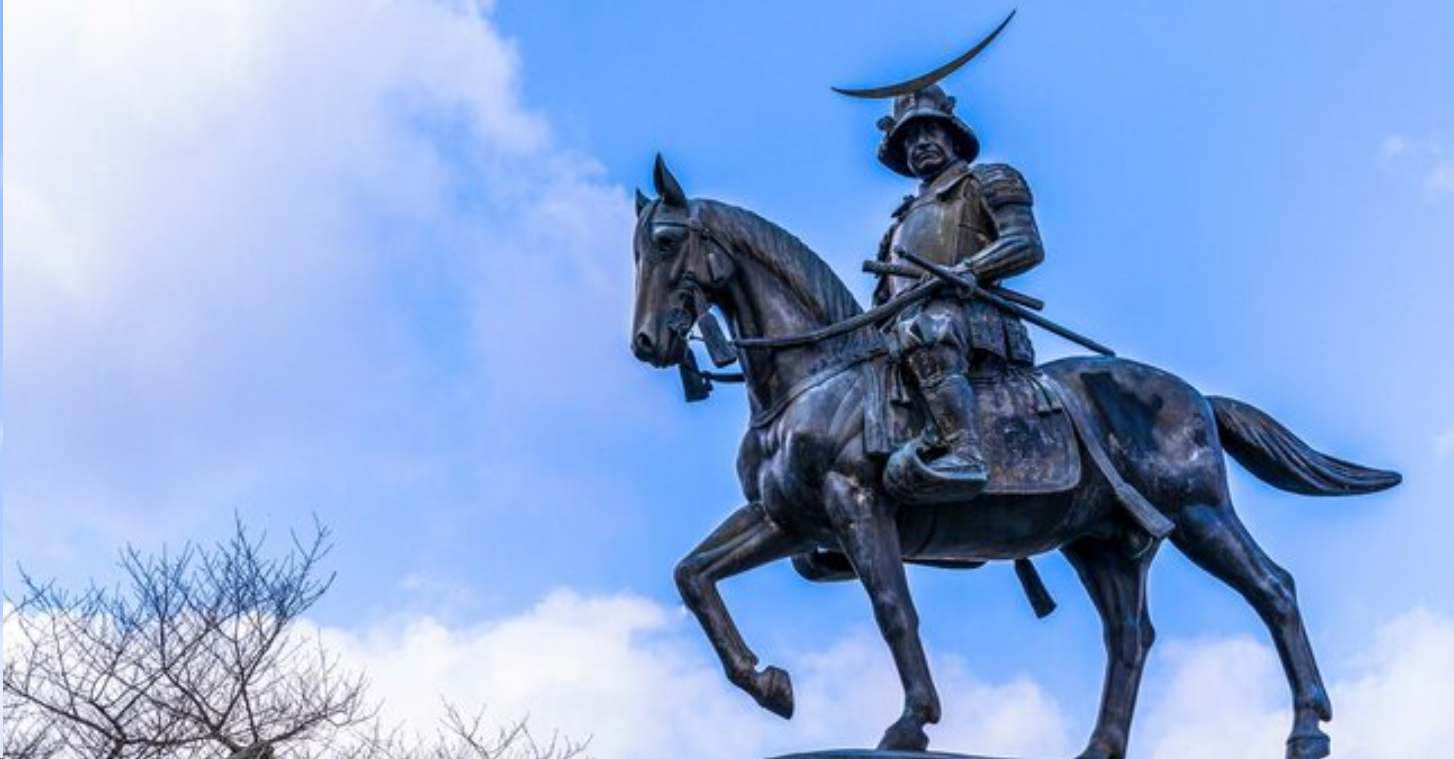
\includegraphics[width=0.6\linewidth]{img/datemasamunezou}
	\label{fig:datemasamunezou}
\end{figure}

政宗の政治的な手腕は,彼の領地である仙台を発展させることに寄与した.
彼は商業や文化の発展を促進し,仙台を東北地方の中心地として位置づけた.
また,彼はキリスト教の布教にも関心を持ち,宣教師を受け入れるなど,国際的な視野を持った人物でもあった.
\newpage

\subsection*{食文化}
\addcontentsline{toc}{subsection}{食文化}

仙台の\textbf{ずんだ}と\textbf{牛タン}は,地域の食文化において非常に重要な役割を果たしている.
これらの料理は,仙台の歴史や文化と深く結びついており,観光客にも人気がある.

\begin{figure}[H]
	\centering
	\begin{minipage}[b]{0.49\columnwidth}
		\centering
		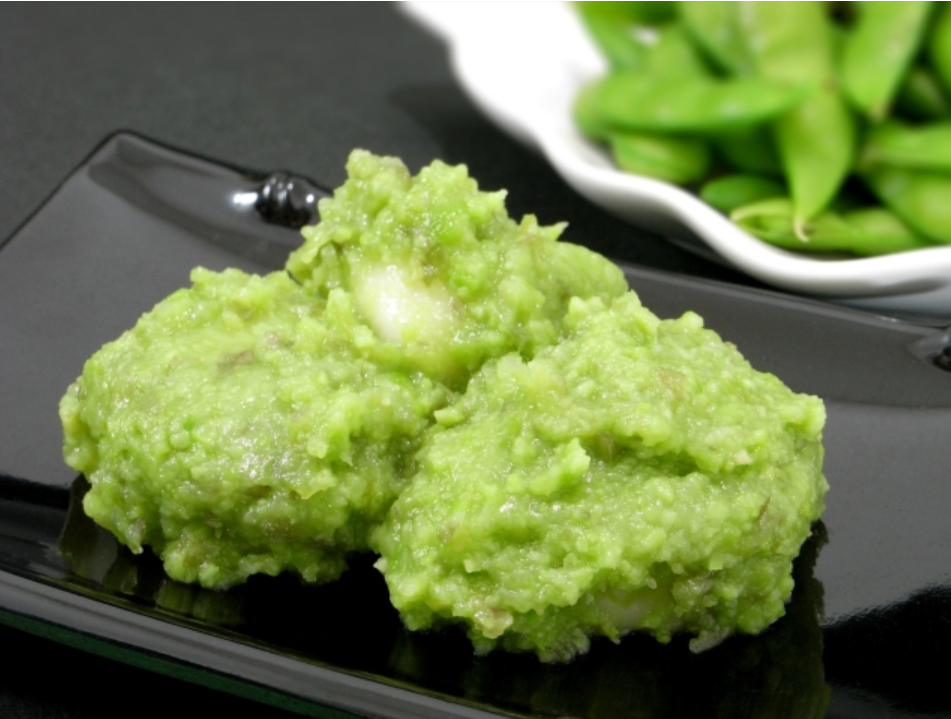
\includegraphics[width=0.9\columnwidth]{img/zundamochi.png}
		\label{fig:zundamochi}
	\end{minipage}
	\begin{minipage}[b]{0.49\columnwidth}
		\centering
		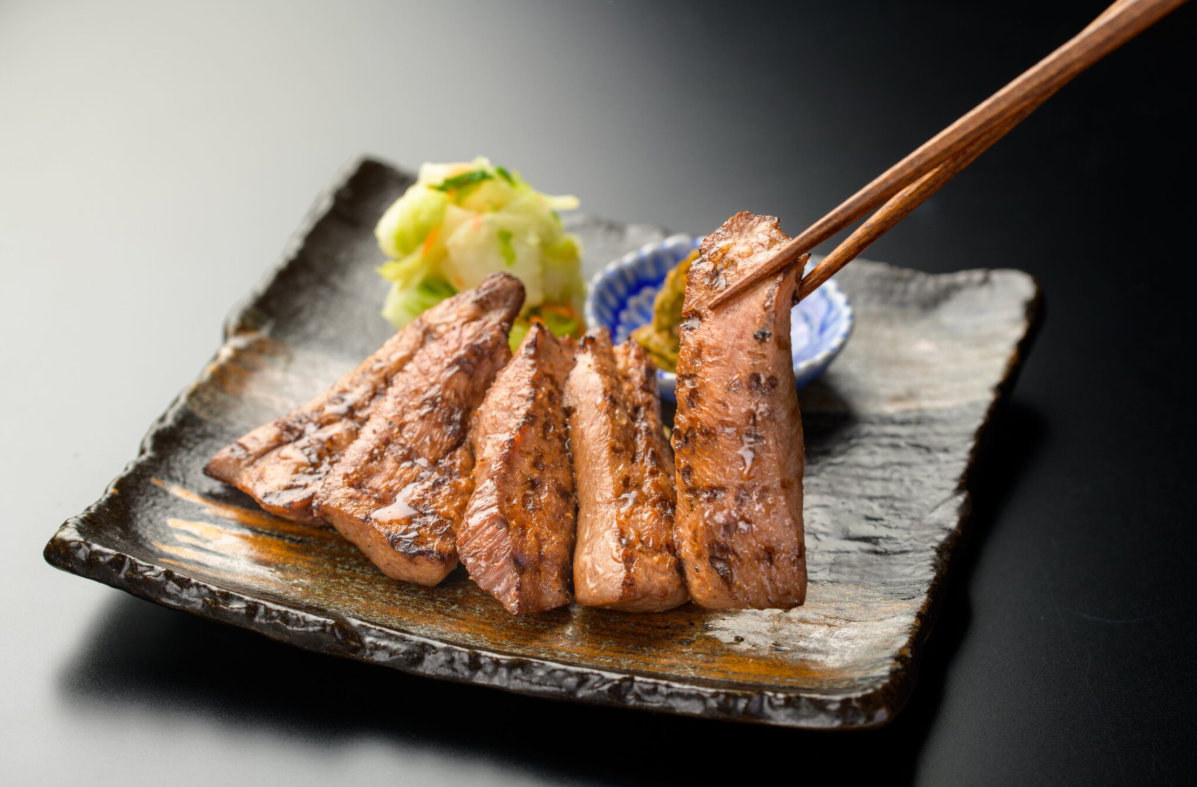
\includegraphics[width=0.9\columnwidth]{img/gyutan-yaki.png}
		\label{fig:gyutan-yaki}
	\end{minipage}
\end{figure}

\subsubsection*{ずんだの歴史}
ずんだは,主に枝豆を使ってペーストで,甘さと独特の風味が特徴である.
ずんだの起源は江戸時代に遡るとされ,当初は農作業の合間に食べられていたと考えられる.
特に,仙台藩の藩士たちが好んで食べていたことから,仙台の名物として広まった.
ずんだの名の由来は,「豆を打つ」の「豆打(づだ)」や,伊達政宗が\ruby{陣太刀}{じんだち}の柄で豆を潰したとの伝説から来た「陣太(じんだ)」が訛って「ずんだ」になったなど,さまざまな説がある.

\subsubsection*{牛タンの歴史}
戦後の1950年代(太平洋戦争が集結し,日本が復興に向けて歩み始めた昭和23年),アメリカの駐在軍が多かった仙台には,大量の牛肉が運び込まれていた.
その中,名店「太助」の初代店主 故・佐野啓四郎氏が洋食で使われていた牛タンの旨さに虜になり,試行錯誤の上,今なお定番となっている\textbf{牛タン焼き}が誕生した.
仙台のローカル定食として誕生した牛タン焼きは,高度経済成長の時代,転勤や出張で仙台にやってきたサラリーマンたちの評判が次第に広がり,マスメディアに取り上げられ,「仙台名物」として全国に広まったとされている.
\newpage

	\newpage
	%\section{おすすめのお土産}

\begin{table}[H]
	\begin{tabular}{ll}
		\textbf{○萩の月} & \textbf{○霜柱} \\
		\begin{minipage}{0.45\textwidth}
			\centering
			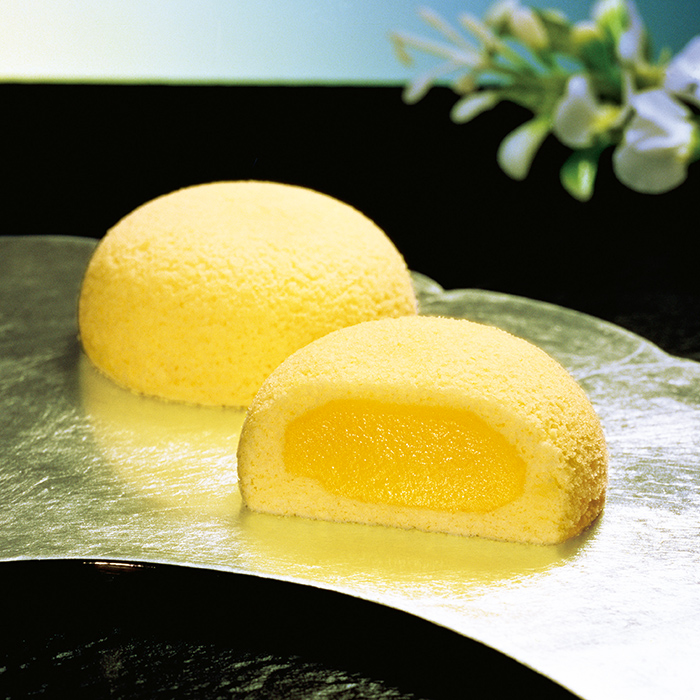
\includegraphics[width=0.7\linewidth]{img/haginotuki}
		\end{minipage} &
		\begin{minipage}{0.45\textwidth}
			\centering
			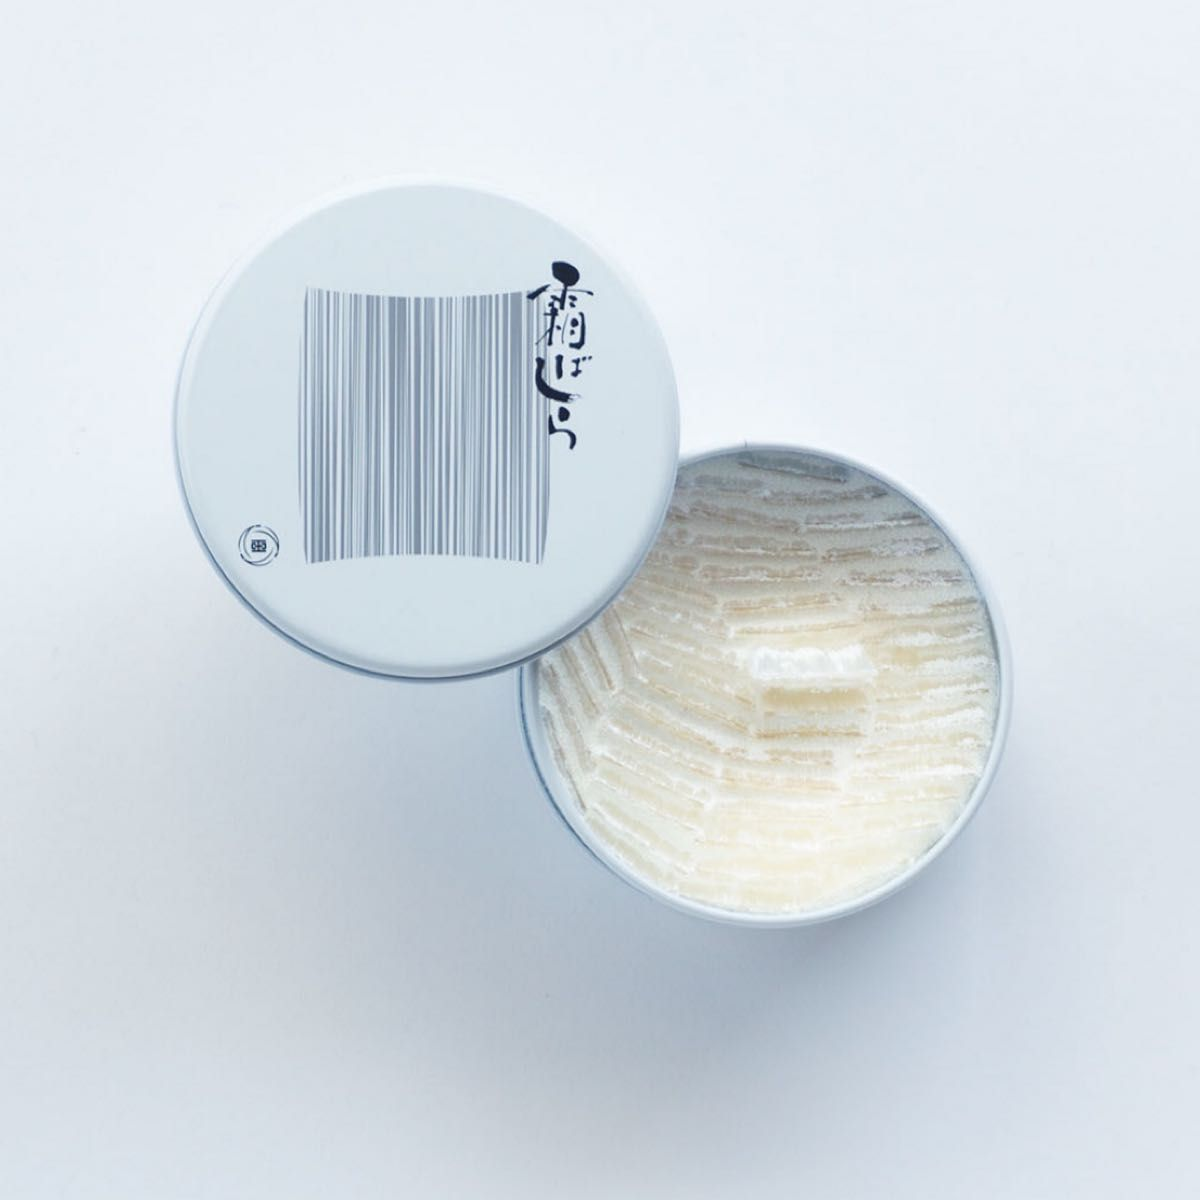
\includegraphics[width=0.7\linewidth]{img/simobashira}
		\end{minipage} \\
		\begin{minipage}{0.45\textwidth}
			\centering
			{\scriptsize{菓匠三全 仙台銘菓}}
		\end{minipage} & 
		\begin{minipage}{0.45\textwidth}
			\centering
			{\scriptsize{九重本舗玉澤}}
		\end{minipage} \\
		\begin{minipage}{0.45\textwidth}
			\centering
			{\scriptsize{6個入り/1500円}}
		\end{minipage} & 
		\begin{minipage}{0.45\textwidth}
			\centering
			{\scriptsize{4320円}}
		\end{minipage} \\
		\textbf{○ずんだ餅} & \textbf{○仙台ラー油} \\
		\begin{minipage}{0.45\textwidth}
			\centering
			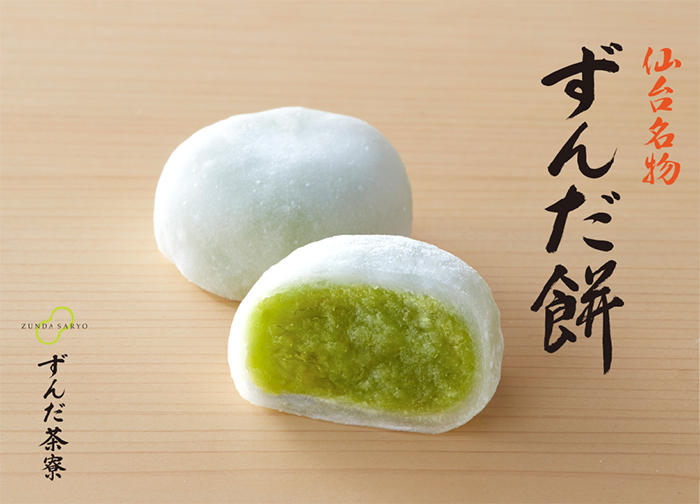
\includegraphics[width=0.7\linewidth]{img/zunda}
		\end{minipage} &
		\begin{minipage}{0.45\textwidth}
			\centering
			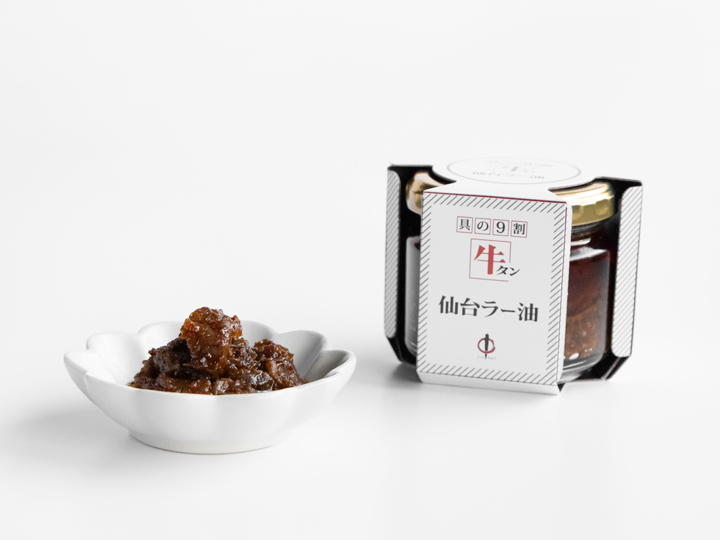
\includegraphics[width=0.7\linewidth]{img/ra-yu}
		\end{minipage} \\
		\begin{minipage}{0.45\textwidth}
			\centering
			{\scriptsize{ずんだ茶寮}}
		\end{minipage} & 
		\begin{minipage}{0.45\textwidth}
			\centering
			{\scriptsize{牛タン専門店 陣中}}
		\end{minipage} \\
		\begin{minipage}{0.45\textwidth}
			\centering
			{\scriptsize{8個入り/1080円}}
		\end{minipage} & 
		\begin{minipage}{0.45\textwidth}
			\centering
			{\scriptsize{100g/900円}}
		\end{minipage} \\
		\textbf{○笹かまぼこ} & \textbf{○日本酒} \\
		\begin{minipage}{0.45\textwidth}
			\centering
			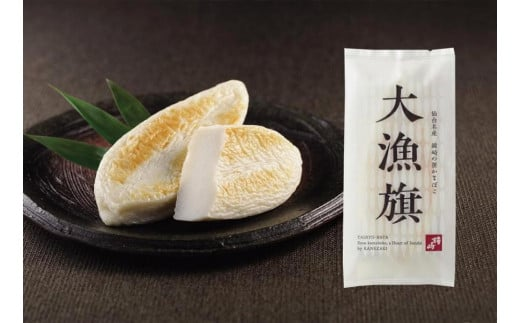
\includegraphics[width=0.7\linewidth]{img/sasakama}
		\end{minipage} &
		\begin{minipage}{0.45\textwidth}
			\centering
			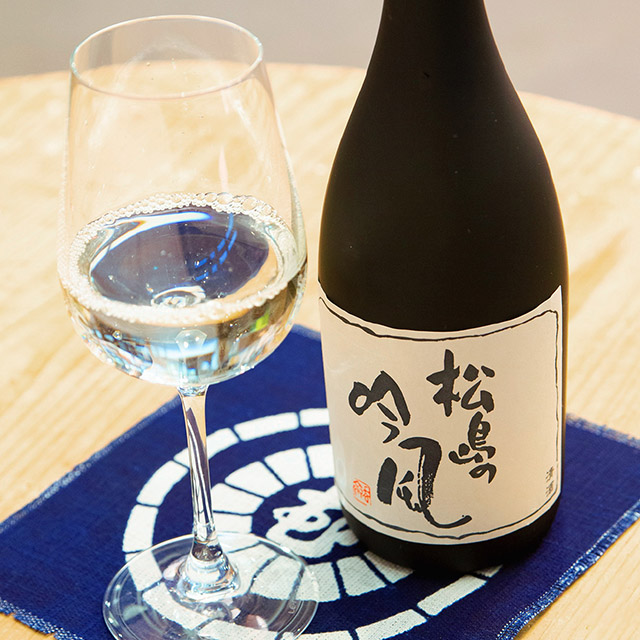
\includegraphics[width=0.7\linewidth]{img/nihonshu}
		\end{minipage} \\
				\begin{minipage}{0.45\textwidth}
			\centering
			{\scriptsize{鐘崎}}
		\end{minipage} & 
		\begin{minipage}{0.45\textwidth}
			\centering
			{\scriptsize{むとう屋 仙台駅店}}
		\end{minipage} \\
		\begin{minipage}{0.45\textwidth}
			\centering
			{\scriptsize{330円}}
		\end{minipage} & 
		\begin{minipage}{0.45\textwidth}
			\centering
			{\scriptsize{}}
		\end{minipage} \\
	\end{tabular}
\end{table}
	\newpage
	%\section{日記}
\centering
\subsection*{第$ n $日目$ m $月$ d $日($ a $)日記}
\addcontentsline{toc}{subsection}{第$ n $日目 $ m $月$ d $日($ a $)日記}
\vspace{0.5cm}
\doublebox{{\scriptsize{チサンイン大村→出島→新地中華街→眼鏡橋→原爆資料館→ハウステンボス}}}
\vspace{0.25cm}

\begin{rightline}
	{\scriptsize{天気:    最高気温:   $ {}^\circ $C}}
\end{rightline}
\begin{table}[H]
	\begin{tabular}{|Wc{10.4cm}|} \hline
		\\ \hline
		\\ \hline
		\\ \hline
		\\ \hline
		\\ \hline
		\\ \hline
		\\ \hline
	\end{tabular}
\end{table}
\begin{figure}[H]
	\begin{minipage}[b]{0.45\hsize}
		\begin{boxnote}
			\vspace{-0.2cm}
			\begin{center}
				\underline{\footnotesize{\textbf{1日目の反省}}}
			\end{center}
			\vspace{-0.4cm}
			%↓この下は1行空けておく↓
			
			\fontsize{12pt}{25pt}\selectfont
			・\\
			・\\
			・\\
			・
		\end{boxnote}
	\end{minipage}
	\hfill
	\begin{minipage}[b]{0.45\hsize}
		\begin{screen}
			\vspace{0.5cm}
			\scriptsize{\textbf{・長崎の今昔を感じたか}}
			\begin{center}
				A \quad B \quad C \quad D
			\end{center}
			\scriptsize{\textbf{・しっかり現状報告できたか}}
			\begin{center}
				A \quad B \quad C \quad D
			\end{center}
			\scriptsize{\textbf{・スムーズに移動できたか}}
			\begin{center}
				A \quad B \quad C \quad D
			\end{center}
			\vspace{0.05cm}
		\end{screen}
	\end{minipage}
\end{figure}

\newpage

\subsection*{第2日目 2月12日(日)日記}
\addcontentsline{toc}{subsection}{第2日目 2月12日(日)日記}
\vspace{0.5cm}
\centering
\doublebox{ハウステンボス}
\vspace{0.25cm}

\begin{rightline}
	{\scriptsize{天気:    最高気温:   $ {}^\circ $C}}
\end{rightline}
\begin{table}[H]
	\centering
	\begin{tabular}{|Wc{10.4cm}|} \hline
		\\ \hline
		\\ \hline
		\\ \hline
		\\ \hline
		\\ \hline
		\\ \hline
		\\ \hline
	\end{tabular}
\end{table}

\begin{figure}[H]
	\begin{minipage}[b]{0.45\hsize}
		\begin{boxnote}
			\vspace{-0.2cm}
			\begin{center}
				\underline{\footnotesize{\textbf{2日目の反省}}}
			\end{center}
			\vspace{-0.4cm}
			%↓この下は1行空けておく↓
			
			\fontsize{12pt}{25pt}\selectfont
			・\\
			・\\
			・\\
			・
		\end{boxnote}
	\end{minipage}
	\hfill
	\begin{minipage}[b]{0.45\hsize}
		\begin{screen}
			\vspace{0.5cm}
			\scriptsize{\textbf{・吝嗇しすぎなかったか}}
			\begin{center}
				A \quad B \quad C \quad D
			\end{center}
			\scriptsize{\textbf{・ハウステンボスの評価は}}
			\begin{center}
				A \quad B \quad C \quad D
			\end{center}
			\tiny{\textbf{・相手へ5年間の感謝の気持ちを伝えられたか}}
			\begin{center}
				A \quad B \quad C \quad D
			\end{center}
			\vspace{0.05cm}
		\end{screen}
	\end{minipage}
\end{figure}

\newpage

\subsection*{第3日目 2月13日(月)日記}
\addcontentsline{toc}{subsection}{第3日目 2月13日(月)日記}
\vspace{0.5cm}
\centering
\doublebox{ハウステンボス→九十九島パールシーリゾート→岡崎}
\vspace{0.25cm}

\begin{rightline}
	{\scriptsize{天気:    最高気温:   $ {}^\circ $C}}
\end{rightline}
\begin{table}[H]
	\centering
	\begin{tabular}{|Wc{10.4cm}|} \hline
		\\ \hline
		\\ \hline
		\\ \hline
		\\ \hline
		\\ \hline
		\\ \hline
		\\ \hline
	\end{tabular}
\end{table}

\begin{figure}[H]
	\begin{minipage}[b]{0.45\hsize}
		\begin{boxnote}
			\vspace{-0.2cm}
			\begin{center}
				\underline{\footnotesize{\textbf{3日目の反省}}}
			\end{center}
			\vspace{-0.4cm}
			%↓この下は1行空けておく↓
			
			\fontsize{12pt}{25pt}\selectfont
			・\\
			・\\
			・\\
			・
		\end{boxnote}
	\end{minipage}
	\hfill
	\begin{minipage}[b]{0.45\hsize}
		\begin{screen}
			\vspace{0.5cm}
			\scriptsize{\textbf{・遊覧船は楽しかったか}}
			\begin{center}
				A \quad B \quad C \quad D
			\end{center}
			\scriptsize{\textbf{・しっかり現状報告できたか}}
			\begin{center}
				A \quad B \quad C \quad D
			\end{center}
			\scriptsize{\textbf{・司温は今日も可愛かったか}}
			\begin{center}
				A+\quad	A \quad B \quad C \quad D
			\end{center}
			\vspace{0.05cm}
		\end{screen}
	\end{minipage}
\end{figure}
	\newpage
	%\paragraph{Memo}

	
\end{document}